\chapter{Machine Learning Methods Applied to Synthetic Ion Acceleration Data} \label{ch:5}

This chapter details the work I did developing and investigating a synthetic dataset based on a model by Fuchs\cite{Fuchs_2005_Nat}.

\section{Modified Fuchs et. al. Model}

In this section, I will describe the model from which we generated the synthetic datasets\cite{Desai_2024_CPP,Desai_2024_arX}. First, the expansion of a plasma into a vacuum\cite{Mora_2003_PRL} is used to determine the maximum proton energy and the number of accelerated protons per unit energy $\frac{dN}{dE}$. Following Fuchs\cite{Fuchs_2005_Nat}, we introduce define the acceleration time in proportion to the pulse duration of the laser and adopt a scaling (e.g. \cref{eq:wilks}) to relate hot electron temperature to the ponderomotive potential. This, in combination with other empirical estimates, allows calculating a proton energy spectrum from up to 7 parameters: main pulse intensity, contrast, wavelength, pulse duration, target thickness, target focal position, and laser spot size.

\subsection{Plasma Expansion into a Vacuum}

This model was developed by Mora\cite{Mora_2003_PRL} in 2003 who built off of earlier efforts\cite{Crow_1975_JPP,Kishimoto_1983_PoF} in examining an isothermal expansion model. The model begins with the assumption that ions are contained in the semi-infinite interval $n_i = n_{i0}$ for $x < 0$ and no ions initially in the vacuum region for $x > 0$. The electrons are distributed according to the boltzmann relation given by \cref{eq:boltzmann} where $n_{e0} = n_e(x = -\infty)$ is the electron density in the unperturbed plasma. Through this relation, $\phi(-\infty) = 0$. The initial electron density is related to the ion density $n_{e0} = Z n_{i0}$ where $Z$ is the ion charge number for a fully ionized plasma. The potential also satisfies the Poisson equation \cref{eq:poisson} where $\rho/m = - e (n_e - Z n_i)$ is the mass density of the electrons. The solution of \cref{eq:poisson} at $t=0$ is found by integration\cite{Crow_1975_JPP} (where $E \equiv -\frac{d\phi}{dx}$) as 

\begin{equation}
	\frac{1}{2} \epsilon_0 E^2 = n_{e0} k_B T_e
	\begin{cases}
		\exp(\frac{e \phi}{k_B T_e} - 1 - \frac{e \phi}{k_B T_e}) & \mbox{if x < 0} \\
		\exp(\frac{e \phi}{k_B T_e}) & \mbox{if x > 0} \label{eq:crow_field}
	\end{cases}
\end{equation} 
From enforcing continuity of \cref{eq:crow_field} at $x=0$ (the location of the ion front initially) we determine $\phi = -k_B T_e / e$ to arrive at  

\begin{equation}
	E_{front,0} = \sqrt{\frac{2}{\exp(1)}} E_0
\end{equation}
where $E_0 \equiv \sqrt{n_{e0} k_B T_e / \epsilon_0}$. To get an estimate of the electric field at the ion front when $t > 0$ we need to consider what the characteristic time scale for ion motion is: the plasma ion frequency $\omega_{p,i}$

\begin{equation}
	\omega_{p,i} \equiv \sqrt{\frac{Z n_{e0} e^2}{m_i \epsilon_0}}	\label{eq:omegapi}
\end{equation} 
which is analogous to \cref{eq:omegape} So, in relation to the time-scale of plasma ion oscillations, a long time would refer to $\omega_{p,i} t \gg 1$. The ion fluid sound speed $c_s$ is given by 

\begin{equation}
	c_s = \sqrt{\frac{Z k_B T_e}{m_i}} \label{eq:soundspeed}
\end{equation}
and which is very similar to \cref{eq:vthermal} Using the definition of the debye length (\cref{eq:debye}) and sound speed $c_s$ we can re-express \cref{eq:omegapi} as 

\begin{equation}
	\omega_{p,i} t = \sqrt{\frac{Z k_B T_e}{m_i}} \sqrt{\frac{n_{e0} e^2}{\epsilon_0 k_B T_e}} t = (c_s t) (\lambda_{D0})
\end{equation}
where $\lambda_{D0}$ is the initial Debye length and $c_s$ is the ion sound speed. As we know from \cref{ch:2}, when $\lambda_D$ is smaller than the characteristic length scale of a system, the quasi-neutrality condition for a plasma is satisfied. In this case, the length scale would be $c_s t$ and we can show that asserting the condition $\omega_{p,i} t > 1$ is equivalent to $\lambda_D < c_s t$. We can continue by incorporating equations of continuity and the Lorentz force (\cref{eq:lorentz}) which can be expressed as 

\begin{subequations}
	\begin{align}
		\frac{\partial n_i}{\partial t} + v_i \frac{\partial n_i}{\partial x} &= - n_i \frac{\partial v_i}{\partial x} \label{eq:continuity} \\
		\frac{\partial v_i}{\partial t} + v_i \frac{\partial v_i}{\partial x} &= -\frac{Z e}{m_i} \frac{\partial V}{\partial x} \label{eq:lorentz_mora}
	\end{align}
\end{subequations}
This set of fluid equations can be solved numerically with the initial conditions for $n_i$, $E$, and $v_i = 0$, but it is more instructive to consider a ``self-similar solution'' that describes the ions moving with speed 
\begin{equation}
	v_i = c_s + x/t \label{eq:selfsimilarvelocity}
\end{equation}
for $x + c_s t > 0$. It is self-similar in the sense that the specific length and time scales are not important, only their ratio $x/t$. In this self-similar region, quasi-neutrality is maintained and the expanding electron density can be expressed as

\begin{equation}
	n_e = Z n_i = n_{e 0} \exp(-\frac{x}{c_s t} - 1) \label{eq:selfsimilardensity}
\end{equation} 
By combining \cref{eq:continuity,eq:lorentz_mora,eq:selfsimilarvelocity,eq:selfsimilardensity}, we can arrive at a solution for the self-similar electric field in this quasi-neutral region

\begin{equation}
	E_{SS} = \frac{m_i c_s}{Z e t} = \frac{k_B T_e}{e c_s t} = \frac{E_0}{\omega_{p,i} t} \label{eq:selfsimilarefield}
\end{equation}
Physically, we can interpret this as a sheet of positive charge $\sigma = \epsilon_0 E_{SS}$ at $x = - c_s t$ and a sheet of negative charge $-\sigma$ at the plasma edge. The location of this plasma edge (i.e. the location of the ion front) can be roughly obtained by equating the local Debye length $\lambda_D = \lambda_{D0} \sqrt{n_{e0}/n_e}$ to the scale length $c_s t$.

\begin{equation}
	x_{i, front} = c_s t [2 \ln(\omega_{p,i} t) - 1] \label{eq:mora_xfront}
\end{equation} 
and the ion velocity at the front can also be obtained 

\begin{equation}
	v_{i, front} = 2 c_s \ln(\omega_{p,i} t)
\end{equation}
The ion velocity can plug back into \cref{eq:lorentz_mora} to find out that $E_\text{front,SS} = 2 E_{SS}$. Mora found an approximate solution to $E_{front}$ that matches $E_\text{front,0}$ and $E_\text{front,SS}$ in their respective cases ($t = 0$ and $\omega_{p,i} t \gg 1$) as 

\begin{equation}
	E_{front} \simeq \frac{2 E_0}{\sqrt{2 \exp(1) + (\omega_{p,i} t)^2}}
\end{equation}

\begin{figure}
	\centering 
	\subfloat{
		\label{fig:fig1_mora}
		\includegraphics[width=0.5\linewidth]{planning/images/fig1_mora.PNG}
	}
	\subfloat{
		\label{fig:fig2_mora}
		\includegraphics[width=0.5\linewidth]{planning/images/fig2_mora.PNG}
	}
	\caption{The net charge density (left) as a function of position $x / c_s t$ and normalized electric field $E/E_0$ (right) for $\omega_{pi} t = 50$ taken from Fig 1 and 2 in Mora's Paper\cite{Mora_2003_PRL}. On the right, the self-similar electric field from \cref{eq:selfsimilarefield} is plotted with a dashed line.}
\end{figure}
This formula not only reaches the correct values in the limiting cases, but also effectively interpolates in the intermediary regions (i.e. $\omega_{p,i} t \sim 1$) when compared to a numerical code that solves \cref{eq:continuity,eq:lorentz_mora} without assuming a self-similar solution. In \cref{fig:fig1_mora}, we see the net charge density at some time $\omega_{pi} t = 50$ after the start of a 1D plasma expansion simulation. We can identify the $-2\sigma$ with the fastest expanding electrons and the $+\sigma$ region next to it as the positive ions getting pulled along. In \cref{fig:fig2_mora}, we can see the electric field between these two charged regions peaks $\simeq 2 E_{ss}$. Then, using this formula with $\cref{eq:lorentz_mora}$, we can determine the ion front velocity as 

\begin{equation}
	v_{i,front} = 2 c_s \ln(\tau + \sqrt{\tau^2 + 1})	
\end{equation}
where we've defined a normalized acceleration time $\tau \equiv \omega_{p,i} t / \sqrt{2 \exp(1)}$. Additionally, in the limit $\omega_{p,i} t \gg 1$, \cref{eq:mora_xfront} becomes

\begin{equation}
	x_{i, front} \simeq c_s t [2 \ln(\omega_{p,i} t) + \ln(2) - 3] \label{eq:mora_xfront_simple}
\end{equation}
The per-ion kinetic energy can now be calculated as

\begin{align}
	\mathcal{E} \equiv \frac{1}{2} m_i v_{i,front}^2 &= 2 m_i c_s^2 \ln(\tau + \sqrt{\tau^2 + 1})^2  \nonumber\\
	&= 2 Z k_B T_{e} \ln(\tau + \sqrt{\tau^2 + 1})^2 \label{eq:mora_maxE}
\end{align}
Using \cref{eq:selfsimilardensity}, we can determine the number of accelerated ions between $x = -c_s t$ and $x = x$ as

\begin{equation}
	N_i \equiv \int_{-c_s t}^{x} n_i(x') dx' = n_{i0} c_s t [1 - \exp(-\frac{x}{c_s t} - 1)]
\end{equation}
and using \cref{eq:selfsimilarvelocity}, we can show that this is equivalent to 

\begin{equation}
	N_i(x) = n_{i0} c_s t [1 - \exp(-\sqrt{\frac{2 \mathcal{E}}{\mathcal{E}_0}})] \label{eq:numprotons}
\end{equation}
where $\mathcal{E}_0 \equiv Z k_B T_e$. Now that the number of ions is expressed in terms of the energy $\mathcal{E}$, we can determine the number of accelerated ions per unit energy (per unit surface) as 

\begin{equation}
	\frac{d N}{d \mathcal{E}} = \frac{n_{i0} c_s t}{\sqrt{2 \mathcal{E} \mathcal{E}_0}} \exp(-\sqrt{\frac{2 \mathcal{E}}{\mathcal{E}_0}}) \label{eq:dNdE}
\end{equation}
	
\subsection{Modified Fuchs Model} \label{sec:fuchsv1}

When $\tau \rightarrow \infty$, \cref{eq:mora_maxE} diverges to $\infty$. This is an inherent limitation of the isothermal fluid model, and different models are able to avoid this issue\cite{Mora_2005_PRE,Passoni_2010_NJoP,Schreiber_2006_PRL}. However, a simple fix to this model involves assuming that this acceleration time is finite and proportional to the pulse duration. Physically, it makes sense that the protons are only getting accelerated on the timescale of  laser-target interactions. This is the approach taken by Fuchs\cite{Fuchs_2005_Nat} and he expresses \cref{eq:mora_maxE} as 

\begin{equation}
	E_\text{max} = 2 k_B T_h [\ln(t_p + \sqrt{t_p^2 + 1})]^2 \label{eq:fuchs_maxE}
\end{equation}
where $\tau \equiv \omega_{p,i} t_\text{acc} / \sqrt{2 \exp(1)}$ just like the Mora model. We've also set $Z=1$ to signify that we are looking for hydrogen ions (i.e. protons) The crucial difference is that we express the acceleration time as 

\begin{equation}
	t_\text{acc} \approx 1.3 \tau_\text{FWHM} \label{eq:fuchs_multiplier}
\end{equation}
One can assume that the absorption fraction of hot electrons $\eta$ (with respect to the total laser energy $E_L$) is given by $\eta_e = 1.2 \times 10^{-15} I^{0.74} \text{ W cm}^{-2}$ with a maximum of 0.5, determined from empirical scalings (e.g. see fig. 3 from Key\cite{Key_1998_PoP}). Additionally, the average energy of the hot electrons is set by the Wilks scaling \cref{eq:wilks}. Putting this together, 

\begin{equation}
	N_e = \eta_e \frac{E_L}{T_h}
\end{equation}
would be the total number of hot electrons accelerated into the target. These electrons spread out in a roughly cylindrical volume of area $S_\text{sheath}$ and length $c \tau{fwhm}$ where the circular sheath cross section can be estimated by $S_\text{sheath} = \pi (r_0 + d \tan(\theta))^2$. Here, $r_0 = w(x) \frac{\sqrt{2 \ln(2)}}{2}$ is half of the (spatial) full width at half maximum of the intensity distribution at position $x$. The effective radius of the sheath has an additional factor of $d \tan(\theta)$ where $d$ is the initial target thickness and $\theta$ is the half-angle divergence of the hot electron within the target (taken as $\theta = 25^\circ$). As a result, the hot electron number density can be expressed as 
	
\begin{equation}
	n_{e0} = \frac{N_e}{c \tau_\text{fwhm} S_\text{sheath}}
\end{equation}
With an estimate of the hot electron density, the proton spectrum can now be computed from \cref{eq:dNdE} as 

\begin{equation}
	\frac{dN}{dE} = N_0 \frac{\exp(-\sqrt{2 E/k_B T_h})}{\sqrt{2 E k_B T_h}} \label{eq:dNdE_Fuchs}
\end{equation}
where $N_0 \equiv n_{e0} c_s t_\text{acc} S_\text{sheath}$ is defined for convenience. Using a dimensionless scale for energy $\varepsilon \equiv \sqrt{2 E / k_B T_h}$, we can calculate the number of protons and total energy in protons through integrating \cref{eq:dNdE_Fuchs}

\begin{align}
	N &= N_0 (\exp(-\varepsilon_\text{min}) - \exp(-\varepsilon_\text{max})) \label{eq:fuchs_N} \\
	E_\text{tot} &= N_0 \frac{k_B T_h}{2}[\exp(-\varepsilon_\text{min})(2 + \varepsilon_\text{min}(2 + \varepsilon_\text{min})) - \exp(-\varepsilon_\text{max})(2 + \varepsilon_\text{max}(2 + \varepsilon_\text{max}))] \label{eq:fuchs_totE}
\end{align}
where $\varepsilon_\text{min} = \sqrt{2 E_\text{min} / k_B T_h}$ defines a minimum energy cutoff ($\varepsilon_\text{max}$ is analogous and chosen by \cref{eq:fuchs_maxE}). Furthermore, we can calculate the average proton energy by dividing \cref{eq:fuchs_N} from \cref{eq:fuchs_totE}

\begin{equation}
	E_\text{avg} \equiv \frac{E_\text{tot}}{N}
\end{equation}
The combination of \cref{eq:fuchs_maxE,eq:dNdE_Fuchs} have been tested across many of the early TNSA experiments of the early 2000s for a wide range of laser intensities and pulse durations with good accuracy (see fig. 4 from Fuchs\cite{Fuchs_2005_Nat}).

\subsection{Further Model Modifications} \label{sec:fuchsv2}
When restricted to a particular laser system, the wavelength, pulse duration, and spot size are fixed. Considering the model in \cref{sec:fuchsv1}, only three adjustable parameters would be of interest -- target thickness $d$, peak intensity $I_0$ and target focal position $x$. To introduce complexity into our model, we wanted to consider the effect that a pre-expanded target would have on the proton acceleration. The pre-expansion may enhance the hot electron generation, but expansion on the rear side of the target would reduce the effectiveness of the TNSA process. We incorporate this effect by allowing the laser to have a finite contrast $\kappa$ which relates the intensity of the main laser pulse $I_0$ to the intensity of a secondary laser pulse $I_\text{pre}$ as $I_\text{pre} = \kappa$. This pre-pulse is treated as a spike in intensity that occurs $t_0$ before the arrival of the main pulse. The pre-expanded target would have a new effective thickness given by 

\begin{equation}
	d_\text{eff} = d + 2 c_s t_0 \label{eq:d_eff}
\end{equation}
where $c_s$ is the ion sound speed from \cref{eq:soundspeed} in which the target is expanding outwards from both sides. Here $T_e$ is the temperature due to the pre-pulse and can be calculated by assuming that $T_e \propto I$ and that an intensity of $10^{12} \text{ W cm}^{-2}$ produces electron temperatures of $T_\text{pre,0} = 50$ eV. Since $n_e$ decreases as $d$ gets larger and $\omega_{p,i} \propto \sqrt{n_e}$, \cref{eq:fuchs_maxE} is inversely proportional to the target thickness. So, a larger prepulse with a longer time to expand $t_0$ will see a higher effective target thickness. Furthermore, when the target is off focus, the effective pre-pulse intensity on target is less which results in less expansion.

In addition, some of the main pulse energy can be depleted by traveling through the underdense region of this new pre-expanded target. These effects will be referred to as \emph{pump depletion} and are inspired by arguments from Decker\cite{Decker_1996_PoP}. Decker describes pump depletion as an ``etching'' process where traveling through the plasma causes wavefront edge to recede at a speed given by the ``etching velocity'' 

\begin{figure}
	\centering 
	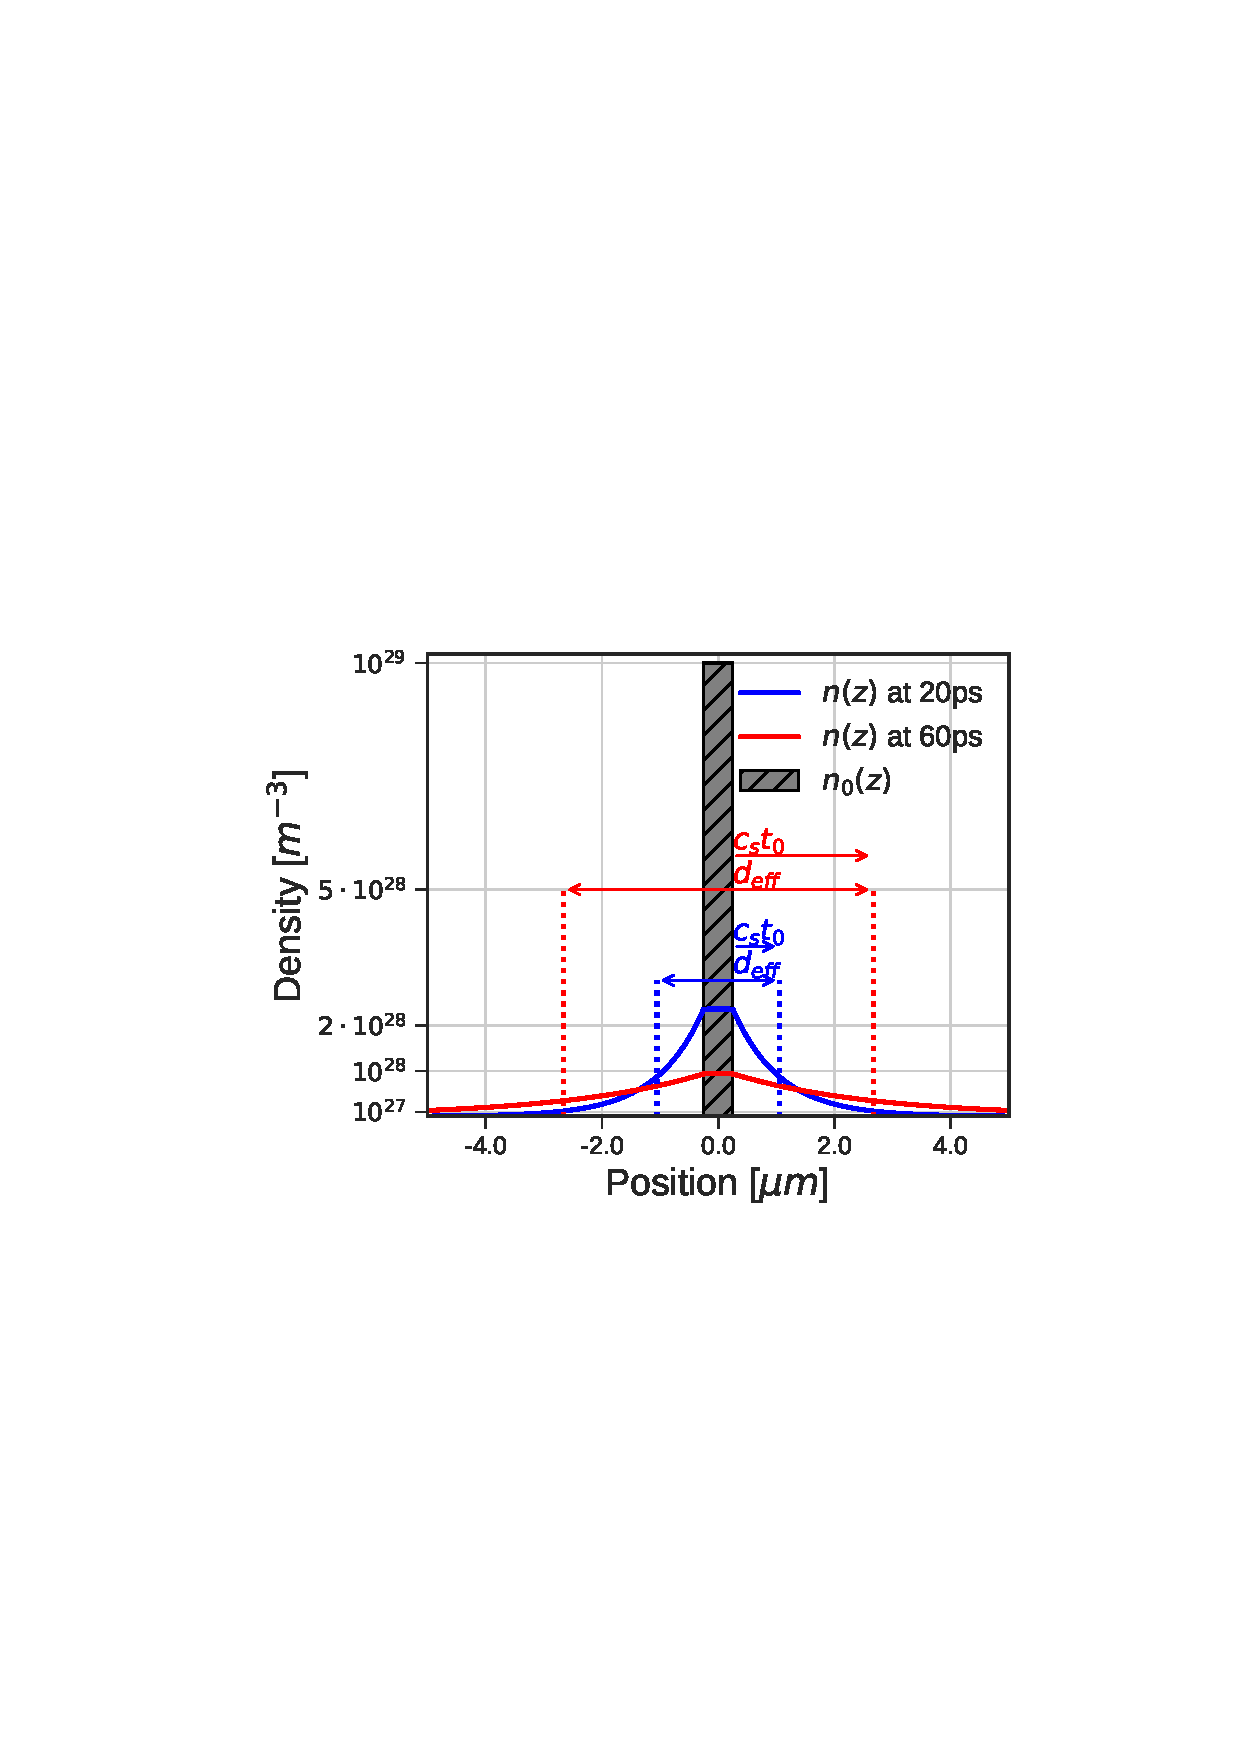
\includegraphics[width=0.6\linewidth]{planning/images/density_profile.png}
	\caption{The electron density profile of the pre-expanded target is depicted for various times $t_0$. In this figure, $n(0) \equiv n_\text{max}$. Taken from Desai et al.\cite{Desai_2024_arX} where $z$ was used as the distance along the laser axis instead of $x$ as done in this work. }
	\label{fig:density_profile}
\end{figure}
\begin{equation}
	v_\text{etch} = (\omega_{p,e}/\omega)^2 c \label{eq:vetch}
\end{equation}
Note that this speed continuously changes throughout the exponential-scale electron density which falls off like $n \sim \exp(-x/c_s t_0)$ on both sides of the target (see \cref{fig:density_profile} for a visual). Due to conservation of particle number, if the target expands, the maximum density $n\text{max}$ will also lower and is given by $n_\text{max} = \frac{n_{e0} d}{d_\text{eff}}$. We can integrate $v_\text{etch}$ with respect to time, but it is more convenient in terms of the position since we know the range over which the under-dense plasma exists. The plasma edge $x_f$ is given by \cref{eq:mora_xfront_simple} and we will integrate up to the location of the critical density $x_0 = c_s t_0 (\ln(n_\text{max}) - \ln(n_c))$. Utilizing the change of variables $dx = c dt$ (due to the pulse traveling at the speed of light $c$), the ``etching distance'' can be calculated as\cite{Desai_2024_arX} 

\begin{equation}
	L_\text{etch} \equiv \int_{x_0}^{x_f} v_\text{etch} \frac{1}{c} dx = \frac{e^2 n_\text{max} c_s t_0}{\epsilon_0 m_e \omega^2} \left( \exp{\left(-\frac{x_0}{c_s t_0}\right)} - \exp{\left(-\frac{x_f}{c_s t_0}\right)} \right)
\end{equation}
Finally, this etching reduces the effective pulse duration by 

\begin{figure}
	\centering 
	\includegraphics[width=0.6\linewidth]{planning/images/energy_dip_morrison.png}
	\caption{The dotted black line shows the maximum proton energy predicted by \cref{eq:fuchs_maxE} with the pump depletion considerations in \cref{sec:fuchsv2} assuming $t_0 = \SI{60}{\pico \second}$, $I_0 = 10^{19} \text{W cm}^{-2}$, $\kappa=10^{-7}$, $d=\SI{0.5}{\micro \meter}$. The red stars indicate the predicted positions of maximum proton energy $\sim \SI{12}{\micro \meter}$. This plot is overlayed on top of an experimental maximum proton energy distribution from Morrison et. al.\cite{Morrison_2018_NJoP}. This figure is taken from Desai et. al.\cite{Desai_2024_arX}.}
	\label{fig:energy_dip_morrison}
\end{figure}
\begin{equation}
	\tau_\text{fwhm,eff} = \tau_\text{fwhm} (1 - \frac{L_\text{etch}}{c \tau_\text{fwhm}}) \label{eq:tau_etch}
\end{equation}
This model, however, is not without its flaws. First, our calculations assume a critical density of a tenth of the amount of the actual critical density. Second, instead of defining $d_\text{eff} = d_0 + 2 x_0$ (which would be the true effective density that remains above critical density), we substitute it with \cref{eq:d_eff}. Third, we modify the multiplier seen in \cref{eq:fuchs_multiplier} from 1.3 to 25 which is a significant departure. Finally, the proportionality $T_e \propto I$ with $T_\text{pre,0} = 50$ eV is chosen arbitrarily. Despite these drawbacks, we obtain model predictions similar to what is seen in \cref{fig:energy_dip_morrison} to account for the maximum proton energy dip at peak focus. The goal of creating this model modification is to add complexity to the underlying physics for the purposes of evaluating the effectiveness of machine learning models, not to invent new physics. 

\section{Results}

\subsection{First Analysis}

\subsection{Second Analysis}

\section{Discussion}